\documentclass[12pt,a4paper]{article}
\usepackage[utf8]{inputenc}
\usepackage{amsmath}
\usepackage{amsfonts}
\usepackage{amssymb}
\usepackage{graphicx}
\usepackage{float}
\usepackage{hyperref}
\usepackage{geometry}
\usepackage{xcolor}
\usepackage{listings}
\usepackage{booktabs}

\geometry{margin=1in}
\hypersetup{
    colorlinks=true,
    linkcolor=blue,
    filecolor=magenta,      
    urlcolor=cyan,
    pdftitle={Problem Set 3 Solutions},
    pdfpagemode=FullScreen,
}

\begin{document}

\begin{figure}[H]
\centering
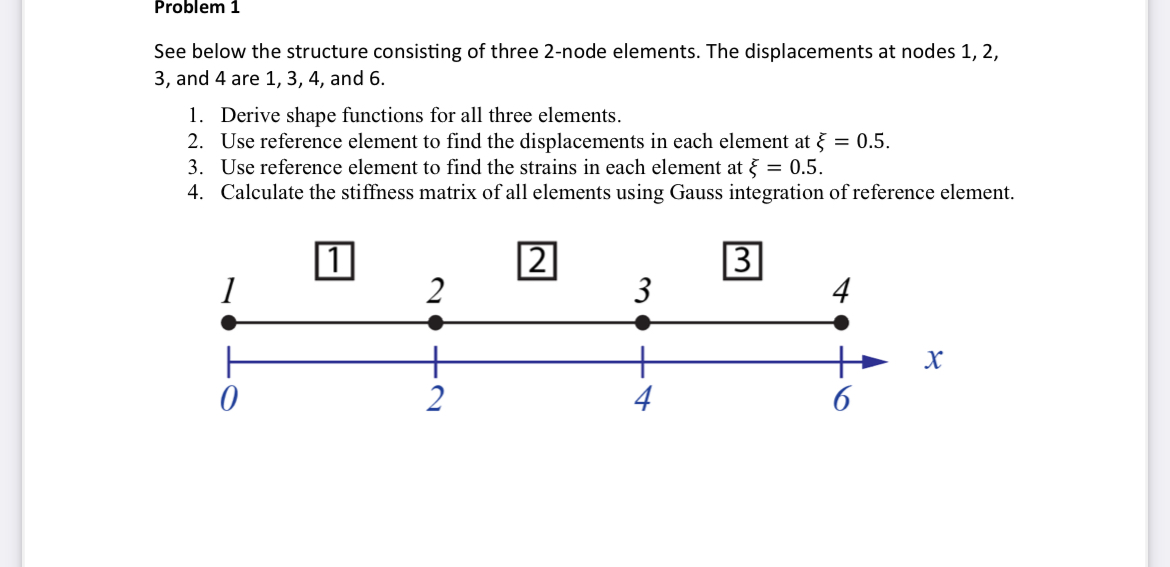
\includegraphics[width=0.9\textwidth]{IMG_5525.jpeg}
\end{figure}

\section{Problem 1}

\subsection{Shape Functions}
For 2-node elements, the shape functions are:
\begin{align}
N_1(\xi) &= \frac{1-\xi}{2} \\
N_2(\xi) &= \frac{1+\xi}{2}
\end{align}
where $\xi$ is the local coordinate ranging from -1 to 1 within each element.

\subsection{Displacements at $\xi = 0.5$}
The displacement at $\xi = 0.5$ in each element is calculated using the shape functions:
\begin{equation}
u(\xi) = N_1(\xi)u_1 + N_2(\xi)u_2
\end{equation}

For $\xi = 0.5$:
\begin{align}
N_1(0.5) &= \frac{1-0.5}{2} = 0.25 \\
N_2(0.5) &= \frac{1+0.5}{2} = 0.75
\end{align}

\subsubsection*{Element 1 (nodes 1-2):}
\begin{align}
u(\xi=0.5) &= 0.25 \times 1 + 0.75 \times 3 \\
&= 0.25 + 2.25 = 2.5
\end{align}

\subsubsection*{Element 2 (nodes 2-3):}
\begin{align}
u(\xi=0.5) &= 0.25 \times 3 + 0.75 \times 4 \\
&= 0.75 + 3.0 = 3.75
\end{align}

\subsubsection*{Element 3 (nodes 3-4):}
\begin{align}
u(\xi=0.5) &= 0.25 \times 4 + 0.75 \times 6 \\
&= 1.0 + 4.5 = 5.5
\end{align}

\subsection{Strains at $\xi = 0.5$}
For 2-node elements, the strain is constant throughout the element:
\begin{equation}
\varepsilon = \frac{u_2 - u_1}{L}
\end{equation}

We need to calculate the strains for each element:

\subsubsection*{Element 1 (L = 2):}
\begin{align}
\varepsilon &= \frac{3 - 1}{2} = 1.0
\end{align}

\subsubsection*{Element 2 (L = 2):}
\begin{align}
\varepsilon &= \frac{4 - 3}{2} = 0.5
\end{align}

\subsubsection*{Element 3 (L = 2):}
\begin{align}
\varepsilon &= \frac{6 - 4}{2} = 1.0
\end{align}

\subsection{Stiffness Matrices}
For a 2-node element with Young's modulus $E$ and cross-sectional area $A$, the stiffness matrix is:
\begin{equation}
\mathbf{k} = \frac{E \cdot A}{L} \begin{bmatrix} 1 & -1 \\ -1 & 1 \end{bmatrix}
\end{equation}

Assuming $E = A = 1$ for simplicity:

\subsubsection*{Element 1 (L = 2):}
\begin{align}
\mathbf{k_1} &= \frac{1 \cdot 1}{2} \begin{bmatrix} 1 & -1 \\ -1 & 1 \end{bmatrix} \\
&= 0.5 \begin{bmatrix} 1 & -1 \\ -1 & 1 \end{bmatrix} \\
&= \begin{bmatrix} 0.5 & -0.5 \\ -0.5 & 0.5 \end{bmatrix}
\end{align}

\subsubsection*{Element 2 (L = 2):}
\begin{align}
\mathbf{k_2} &= \begin{bmatrix} 0.5 & -0.5 \\ -0.5 & 0.5 \end{bmatrix}
\end{align}

\subsubsection*{Element 3 (L = 2):}
\begin{align}
\mathbf{k_3} &= \begin{bmatrix} 0.5 & -0.5 \\ -0.5 & 0.5 \end{bmatrix}
\end{align}

\clearpage
\begin{figure}[H]
\centering
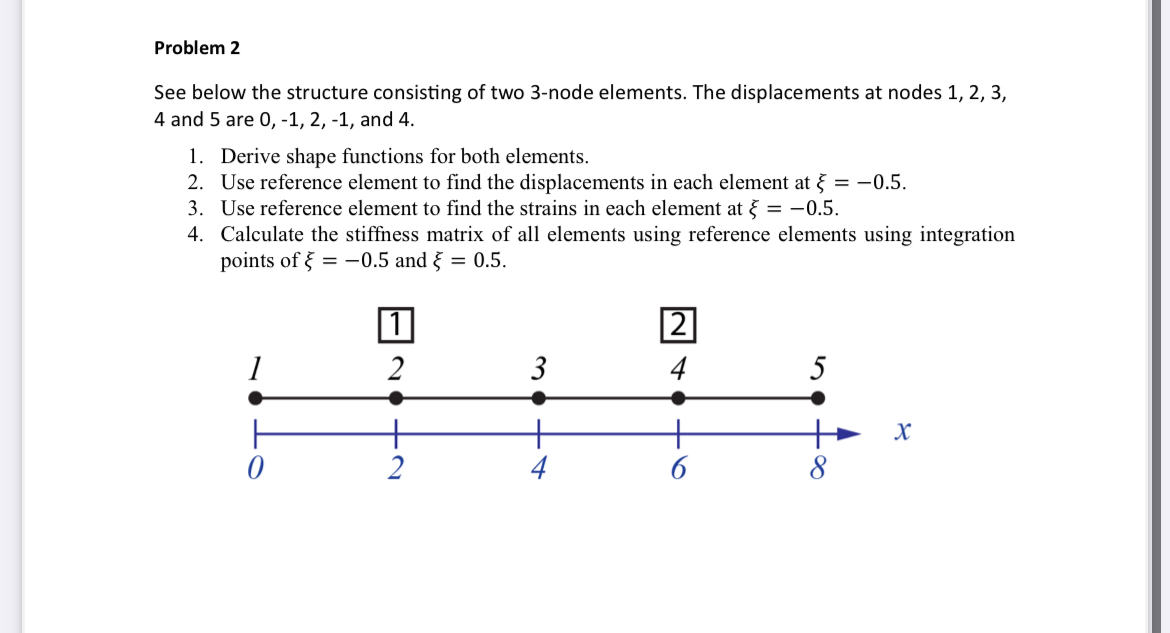
\includegraphics[width=0.9\textwidth]{IMG_5526.jpeg}
\end{figure}

\section{Problem 2}

\subsection{Shape Functions}
For 3-node elements, the shape functions are:
\begin{align}
N_1(\xi) &= \frac{\xi(\xi-1)}{2} \\
N_2(\xi) &= (1+\xi)(1-\xi) \\
N_3(\xi) &= \frac{\xi(\xi+1)}{2}
\end{align}
where $\xi$ is the local coordinate ranging from -1 to 1 within each element, with $\xi = -1, 0, 1$ corresponding to the three nodes.

\subsection{Displacements at $\xi = -0.5$}
The displacement at $\xi = -0.5$ in each element is calculated using the shape functions:
\begin{equation}
u(\xi) = N_1(\xi)u_1 + N_2(\xi)u_2 + N_3(\xi)u_3
\end{equation}

For $\xi = -0.5$:
\begin{align}
N_1(-0.5) &= \frac{-0.5(-0.5-1)}{2} = \frac{-0.5 \times (-1.5)}{2} = \frac{0.75}{2} = 0.125 \\
N_2(-0.5) &= (1+(-0.5))(1-(-0.5)) = 0.5 \times 1.5 = 0.75 \\
N_3(-0.5) &= \frac{-0.5(-0.5+1)}{2} = \frac{-0.5 \times 0.5}{2} = -0.125
\end{align}

\subsubsection*{Element 1 (nodes 1-2-3):}
\begin{align}
u(\xi=-0.5) &= 0.125 \times 0 + 0.75 \times (-1) + (-0.125) \times 2 \\
&= 0 - 0.75 - 0.25 = -1.0
\end{align}

\subsubsection*{Element 2 (nodes 3-4-5):}
\begin{align}
u(\xi=-0.5) &= 0.125 \times 2 + 0.75 \times (-1) + (-0.125) \times 4 \\
&= 0.25 - 0.75 - 0.5 = -1.0
\end{align}

\subsection{Strains at $\xi = -0.5$}
For 3-node elements, the strain varies within the element and is calculated using:
\begin{equation}
\varepsilon = \mathbf{B} \cdot \mathbf{u}, \text{ where } \mathbf{B} = \left[\frac{dN_1}{dx}, \frac{dN_2}{dx}, \frac{dN_3}{dx}\right]
\end{equation}

At $\xi = -0.5$:
\begin{align}
\frac{dN_1}{d\xi} &= \xi - 0.5 = -0.5 - 0.5 = -1.0 \\
\frac{dN_2}{d\xi} &= -2\xi = -2 \times (-0.5) = 1.0 \\
\frac{dN_3}{d\xi} &= \xi + 0.5 = -0.5 + 0.5 = 0.0
\end{align}

The Jacobian for both elements (L = 4):
\begin{equation}
J = \frac{L}{2} = \frac{4}{2} = 2
\end{equation}

Converting to derivatives with respect to $x$:
\begin{align}
\frac{dN_1}{dx} &= \frac{dN_1}{d\xi} \cdot \frac{d\xi}{dx} = \frac{-1.0}{2} = -0.5 \\
\frac{dN_2}{dx} &= \frac{dN_2}{d\xi} \cdot \frac{d\xi}{dx} = \frac{1.0}{2} = 0.5 \\
\frac{dN_3}{dx} &= \frac{dN_3}{d\xi} \cdot \frac{d\xi}{dx} = \frac{0.0}{2} = 0.0
\end{align}

\subsubsection*{Element 1:}
\begin{align}
\varepsilon &= -0.5 \times 0 + 0.5 \times (-1) + 0.0 \times 2 \\
&= 0 - 0.5 + 0 = -0.5
\end{align}

\subsubsection*{Element 2:}
\begin{align}
\varepsilon &= -0.5 \times 2 + 0.5 \times (-1) + 0.0 \times 4 \\
&= -1.0 - 0.5 + 0 = -1.5
\end{align}

\subsection{Stiffness Matrices}
For a 3-node element, the stiffness matrix is calculated using numerical integration:
\begin{equation}
\mathbf{k} = \int\mathbf{B}^T \cdot E \cdot \mathbf{B} \cdot A \cdot \det(J) \, d\xi
\end{equation}

Using integration points $\xi = -0.5$ and $\xi = 0.5$ with equal weights of 1.0 and assuming $E = A = 1$:

For Element 1 at $\xi = -0.5$:
\begin{align}
\mathbf{B}^T &= \begin{bmatrix} -0.5 \\ 0.5 \\ 0 \end{bmatrix} \\
\mathbf{k}_{contribution} &= \begin{bmatrix} -0.5 \\ 0.5 \\ 0 \end{bmatrix} \cdot \begin{bmatrix} -0.5 & 0.5 & 0 \end{bmatrix} \cdot 1 \cdot 1 \cdot 2 \cdot 1 \\
&= \begin{bmatrix} 0.5 & -0.5 & 0 \\ -0.5 & 0.5 & 0 \\ 0 & 0 & 0 \end{bmatrix}
\end{align}

For Element 1 at $\xi = 0.5$:
\begin{align}
\mathbf{B}^T &= \begin{bmatrix} 0 \\ 0 \\ 0.5 \end{bmatrix} \\
\mathbf{k}_{contribution} &= \begin{bmatrix} 0 \\ 0 \\ 0.5 \end{bmatrix} \cdot \begin{bmatrix} 0 & 0 & 0.5 \end{bmatrix} \cdot 1 \cdot 1 \cdot 2 \cdot 1 \\
&= \begin{bmatrix} 0 & 0 & 0 \\ 0 & 0 & 0 \\ 0 & 0 & 0.5 \end{bmatrix}
\end{align}

Combining both contributions for Element 1:
\begin{align}
\mathbf{k_1} &= \begin{bmatrix} 0.5 & -0.5 & 0 \\ -0.5 & 0.5 & 0 \\ 0 & 0 & 0 \end{bmatrix} + \begin{bmatrix} 0 & 0 & 0 \\ 0 & 0.5 & -0.5 \\ 0 & -0.5 & 0.5 \end{bmatrix} \\
&= \begin{bmatrix} 0.5 & -0.5 & 0 \\ -0.5 & 1.0 & -0.5 \\ 0 & -0.5 & 0.5 \end{bmatrix}
\end{align}

Similarly for Element 2:
\begin{align}
\mathbf{k_2} &= \begin{bmatrix} 0.5 & -0.5 & 0 \\ -0.5 & 1.0 & -0.5 \\ 0 & -0.5 & 0.5 \end{bmatrix}
\end{align}

\begin{table}[H]
\centering
\begin{tabular}{lccc}
\toprule
\textbf{Quantity} & \textbf{Element 1} & \textbf{Element 2} & \textbf{Element 3} \\
\midrule
Displacement at $\xi = 0.5$ & 2.5 & 3.75 & 5.5 \\
Strain at $\xi = 0.5$ & 1.0 & 0.5 & 1.0 \\
\bottomrule
\end{tabular}
\caption{Results for Problem 1}
\end{table}

\begin{table}[H]
\centering
\begin{tabular}{lcc}
\toprule
\textbf{Quantity} & \textbf{Element 1} & \textbf{Element 2} \\
\midrule
Displacement at $\xi = -0.5$ & -1.0 & -1.0 \\
Strain at $\xi = -0.5$ & -0.5 & -1.5 \\
\bottomrule
\end{tabular}
\caption{Results for Problem 2}
\end{table}

\end{document}
